\documentclass[12pt]{article}
\usepackage{amsmath}
\usepackage{pgfplots}
\usepackage{graphicx}
\usepackage{float}
\begin{document}
\title{Electrical Engineering 141, Homework 3}
\date{February 1st, 2019}
\author{Michael Wu\\UID: 404751542}
\maketitle

\section*{Problem 1}

\paragraph{a)}

\begin{align*}
    Y(s) &= \frac{K}{\tau s + 1}(R(s) - Y(s))\\
    \left(1+\frac{K}{\tau s + 1}\right)Y(s) &= \frac{K}{\tau s + 1}R(s)\\
    \frac{\tau s + 1 + K}{\tau s + 1} Y(s) &= \frac{K}{\tau s + 1}R(s)\\
    \frac{Y(s)}{R(s)} &= \frac{K}{\tau s + 1 + K}
\end{align*}

\paragraph{b)}

If the input is the unit step function, it will have a Laplace transform of \(\frac{1}{s}\). Then we have
\begin{align*}
    Y(s) &= \frac{K}{s(\tau s + 1 + K)}\\
    &=\frac{K}{s(1+K)}-\frac{K\tau}{(1+K)(\tau s + 1 + K)}
\end{align*}
This has an inverse Laplace transform of
\[y(t) = \frac{K}{1+K}\left(1 - e^{-\frac{(1+K)t}{\tau}}\right)u(t)\]
This looks like the plot shown below.
\begin{center}
    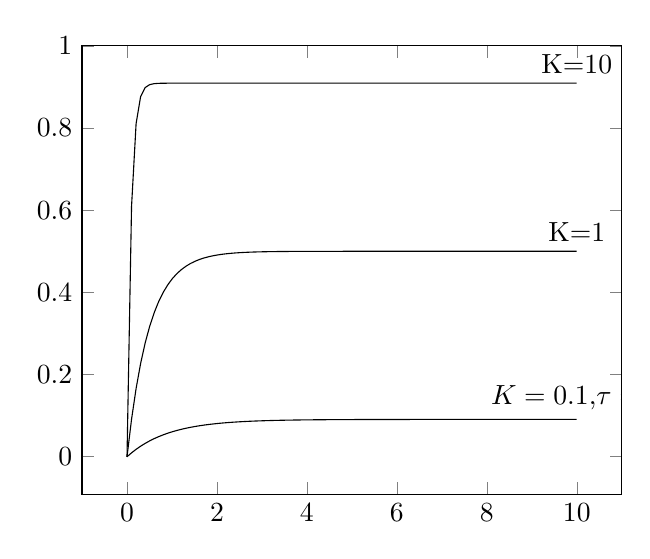
\begin{tikzpicture}
        \begin{axis}[
            domain=0:10,
            samples=100
        ]
            \addplot[black] {0.1/1.1*(1 - exp{-1.1*x})} node[above] {\(K=0.1\),\(\tau=1\)};
            \addplot[black] {1/2*(1 - exp{-2*x})} node[above] {K=1};
            \addplot[black] {10/11*(1 - exp{-11*x})} node[above] {K=10};
        \end{axis}
    \end{tikzpicture}
\end{center}

\paragraph{c)}

The DC gain of this system is \(\frac{K}{1+K}\). The time constant of this system is \(\frac{\tau}{1+K}\).

\paragraph{d)}

The steady state error of this system with the unit step input is \(\frac{1}{1+K}\).

\paragraph{e)}

For a maximum 10\% steady state error we would need to have \(\frac{1}{1+K}=0.1\) which gives \(K=9\). Then can solve the following.
\begin{align*}
    e^{-10\frac{2}{\tau}}&=0.02\\
    -10\frac{2}{\tau}&=\ln(0.02)\\
    \tau &= -\frac{20}{\ln(0.02)}\\
    \tau &=\frac{20}{\ln(50)}\approx 5.112
\end{align*}

\section*{Problem 2}

\paragraph{a)}

It reached 2\% error in 60 seconds. So we can solve the following.
\begin{align*}
    e^{-\frac{60}{\tau}}&=0.02\\
    -\frac{60}{\tau}&=\ln(0.02)\\
    \tau &= -\frac{60}{\ln(0.02)}\\
    \tau &=\frac{60}{\ln(50)}\approx 15.34
\end{align*}
So it has a time constant of approximately 15.34 seconds.

\paragraph{b)}

The output will have a Laplace transform of \(\frac{2}{s^2(\tau s+1)}\). This is equivalent to the following.
\[Y(s)= \frac{2}{s^2}-\frac{2\tau}{ s} + \frac{2\tau^2}{\tau s + 1}\]
This has the following inverse Laplace transform.
\[Y(t)= 2tu(t)-2\tau(1-e^{-\frac{t}{\tau}})u(t)\]
So as time increases, the thermometer temperature will be \(2\tau\) or
\[2\frac{60}{\ln(50)}\frac{1}{60} = 0.5112\]
degrees below the tank temperature.

\section*{Problem 3}

\paragraph{a)}

The poles are located at
\[\frac{-2\zeta\omega_n\pm\sqrt{4\zeta^2\omega_n^2-4\omega_n^2}}{2}=\omega_n(-\zeta\pm\sqrt{\zeta^2-1})\]
Since \(\zeta^2-1\) must be negative in order to have imaginary poles, the minimum value that \(\zeta\) can take
is \(-1\). Note that \(\omega_n\) simply scales the roots by a constant factor. So the \(\zeta\) traces out an arc
in the imaginary plane, while the \(\omega_n\) extends this out radially which leads to the following shape.
\begin{figure}[H]
    \begin{center}
        \includegraphics[width=3.5in]{problem3a.png}
    \end{center}
\end{figure}

\paragraph{b)}

We have that \(\omega_n=\frac{\omega_d}{\sqrt{1-\zeta^2}}\). Then our poles are located at
\[\omega_d\left(-\frac{\zeta}{\sqrt{1-\zeta^2}}\pm j\right)\]
So this looks like the following.
\begin{figure}[H]
    \begin{center}
        \includegraphics[width=3.5in]{problem3b.png}
    \end{center}
\end{figure}

\paragraph{c)}

From the maximum overshoot we have the following.
\begin{align*}
    e^{-\frac{\pi\zeta}{\sqrt{1-\zeta^2}}} &< 0.2\\
    -\frac{\pi\zeta}{\sqrt{1-\zeta^2}} &< \ln(0.2)\\
    \frac{\zeta}{\sqrt{1-\zeta^2}} &> -\frac{\ln(0.2)}{\pi}\\
    \zeta^2 &> (1-\zeta^2)\frac{\ln^2(5)}{\pi^2}\\
    \left(1+\frac{\ln^2(5)}{\pi^2}\right)\zeta^2 &> \frac{\ln^2(5)}{\pi^2}\\
    \zeta &> \frac{\ln(5)}{\sqrt{\pi^2 +\ln^2(5)}}
\end{align*}
From the settling time we have the following.
\begin{align*}
    -\frac{1}{\zeta\omega_n}\ln\left(0.02\sqrt{1-\zeta^2}\right) &< 2\\
    -\frac{1}{2\zeta}\ln\left(0.02\sqrt{1-\zeta^2}\right) &< \omega_n
\end{align*}
This region is left of the following boundary.
\begin{figure}[H]
    \begin{center}
        \includegraphics[width=3.5in]{problem3c.png}
    \end{center}
\end{figure}

\section*{Problem 4}

\paragraph{a)}

The step response has a Laplace transform of
\[\frac{2(1-s)}{s(s+1)(s+2)}\]
which can be rewritten using partial fraction decomposition as follows.
\[\frac{1}{s}-\frac{4}{s+1} + \frac{3}{s+2}\]
This has an inverse Laplace transform of
\[(1-4e^{-t}+3e^{-2t})u(t)\]
which looks like the following plot.
\begin{center}
    \begin{tikzpicture}
        \begin{axis}[
            domain=0:10,
            samples=100
        ]
            \addplot[black] {1-4*exp{-x}+3*exp{-2*x}};
        \end{axis}
    \end{tikzpicture}
\end{center}

\paragraph{b)}

The derivative of the step response at \(t=0\) is
\[\left.4e^{-t}-6e^{-2t}\right|_{t=0}=-2\]

\paragraph{c)}

The step response initially goes downwards, which is unexpected because we would want
the step response to move towards 1, its steady state response. This is most likely
due to the correction for a large move pushing the response in the negative direction.
After a while as the input stays the same, the response moves towards the steady state
value of 1.

\section*{Problem 5}

\paragraph{a)}

Let us find the transfer function for the inner feedback loop.
\begin{align*}
    \Omega(s) &= \frac{100}{0.2s+1}K(X(s)-K_g\Omega(s))\\
    \left(1+KK_g\frac{100}{0.2s+1}\right)\Omega(s)&=\frac{100}{0.2s+1}KX(s)\\
    \frac{\Omega(s)}{X(s)}&=\frac{100K}{0.2s+1+100KK_g}
\end{align*}
Then we can solve for the transfer function of the outer feedback loop.
\begin{align*}
    \Theta(s) &= \frac{100K(\Theta_r(s) -\Theta(s))}{20s(0.2s+1+100KK_g)}\\
    \left(1+\frac{100K}{20s(0.2s+1+100KK_g)}\right)\Theta(s)&=\frac{100K}{20s(0.2s+1+100KK_g)}\Theta_r(s)\\
    \frac{\Theta(s)}{\Theta_r(s)}&=\frac{25K}{s^2+(5+500KK_g)s+25K}
\end{align*}
This is a second order system, so we will try to solve for the following.
\begin{align*}
    5+500KK_g&=2\zeta\omega_n\\
    25K&=\omega_n^2
\end{align*}
This can be rewritten as
\begin{align*}
    K_g&=\frac{2\zeta\omega_n-5}{20\omega_n^2}\\
    K&=\frac{\omega_n^2}{25}
\end{align*}
Then the percentage overshoot yields the following relationship.
\begin{align*}
    e^{-\frac{\pi\zeta}{\sqrt{1-\zeta^2}}} &= 0.1\\
    -\frac{\pi\zeta}{\sqrt{1-\zeta^2}} &= \ln(0.1)\\
    \frac{\zeta}{\sqrt{1-\zeta^2}} &= -\frac{\ln(0.1)}{\pi}\\
    \zeta^2 &= (1-\zeta^2)\frac{\ln^2(10)}{\pi^2}\\
    \left(1+\frac{\ln^2(10)}{\pi^2}\right)\zeta^2 &= \frac{\ln^2(10)}{\pi^2}\\
    \zeta &= \frac{\ln(10)}{\sqrt{\pi^2 +\ln^2(10)}}
\end{align*}
The settling time yields the following relationship.
\begin{align*}
    0.05 &= -\frac{1}{\zeta\omega_n}\ln\left(0.02\sqrt{1-\zeta^2}\right)\\
    \omega_n &= \frac{20}{\zeta}\ln\left(\frac{50}{\sqrt{1-\zeta^2}}\right)\\
    \omega_n &= \frac{20}{\frac{\ln(10)}{\sqrt{\pi^2 +\ln^2(10)}}}\ln\left(\frac{50}{\sqrt{1-\left(\frac{\ln(10)}{\sqrt{\pi^2 +\ln^2(10)}}\right)^2}}\right)\\
    \omega_n &= \frac{20\sqrt{\pi^2 +\ln^2(10)}}{\ln(10)} \ln\left(\frac{50\sqrt{\pi^2 +\ln^2(10)}}{\pi}\right)
\end{align*}
Plugging into the earlier expressions yields the following.
\begin{align*}
    K_g&=\frac{\left(8\ln\left(\frac{50\sqrt{\pi^2 +\ln^2(10)}}{\pi}\right)-1\right)\ln^2(10)}{1600(\pi^2 +\ln^2(10))\ln^2\left(\frac{50\sqrt{\pi^2 +\ln^2(10)}}{\pi}\right)}\approx 0.00041056\\
    K&=\frac{16(\pi^2 +\ln^2(10)) \ln^2\left(\frac{50\sqrt{\pi^2 +\ln^2(10)}}{\pi}\right)}{\ln^2(10)}\approx 779.8
\end{align*}

\paragraph{b)}

I translated my previous results into the following code.
\scriptsize
\begin{verbatim}
K = (16*(pi^2+log(10)^2)*log((50*sqrt(pi^2 +log(10)^2))/pi)^2)/(log(10)^2);
Kg = (8*log(50*sqrt(pi^2 +log(10)^2)/pi)-1)*log(10)^2/(1600*(pi^2+log(10)^2)...
*log(50*sqrt(pi^2+log(10)^2)/pi)^2);
s = tf('s');
H = 25*K/(s^2 + (5+500*K*Kg)*s + 25*K);
set(gcf,'color','w');
step(H);
export_fig problem5b.pdf;
stepinfo(H)
\end{verbatim}
\normalsize
This produced a settling time of 0.0424 seconds and a 10\% overshoot, as expected. The slight error in the
settling time is due to the settling time formula using the envelope only. The real signal settles earlier
due to the sinusoidal term bringing the response within the settling range before the envelope is entirely
within the settling range. The step response is shown below.
\begin{figure}[H]
    \begin{center}
        \includegraphics[width=3.5in]{problem5b.pdf}
    \end{center}
\end{figure}

\section*{Problem 6}

\paragraph{a)}

\paragraph{b)}

\paragraph{c)}

\paragraph{d)}

\paragraph{e)}

\section*{Problem 7}

\section*{Problem 8}

\paragraph{a)}

\paragraph{b)}

\section*{Problem 9}

\paragraph{a)}

\paragraph{b)}

\paragraph{c)}

\end{document}